 \section{Soft-edge clocking}
\label{sec:softedge}

Another proposal has been the use of soft-edge clocking, such as the soft-edge flip-flop (SFF) to increase speed in near-threshold devices by reducing the maximum clock frequency's dependence on critical path delay~\cite{Wieckowski:2008bo}.
 In this design, a traditional D-flip flop is modified to be driven by two offset clocks, generating a short transparency window.
 At the limit where the offset between the clocks is 0, the SFF acts identically to a standard DFF.
 As the offset between the two clocks increases, the SFF's transparency window increases, allowing more time borrowing and allowing the chip to run faster, as shown in Figure~\ref{fig:sff}.
 If the offset becomes too large, functional failures can occur in short paths as signals race through the transparent flip-flops. 
\begin{figure}[thpb]
    \centering
    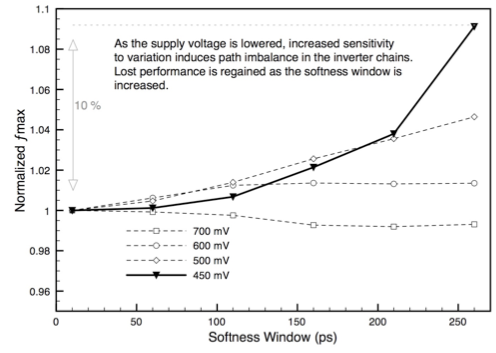
\includegraphics[width=0.4\textwidth]{wieckowski_sff.png}
    \caption{Frequency improvement as SFF transparency increases.~\cite{Wieckowski:2008bo}}
    \label{fig:sff}
\end{figure}

Generating the offset between the two clocks becomes an issue as variability increases.
 The simple method used in the paper of having a chain of inverters would be heavily susceptible to process variations.
As $\sigma_v/\mu$ increases, the variance of the delay through this chain of inverters increases.
Because this delay sets the offset between the two clocks, the increased variance results in a wider range of performance for the SFFs in the design.

